\documentclass[final,acmlarge,draft=false,review=false,nonacm=false]{acmart}
\usepackage[
    type={CC},           % your choice
    modifier={by-sa},    % your choice
    version={4.0},       % your choice
]{doclicense}            % your choice, see \doclicenseThis below


\usepackage{alltt}
\usepackage{latexsym}
\usepackage{array}
%\usepackage{comment}
%\usepackage{makeidx}
%\usepackage{indentfirst}
%\usepackage{verbatim}
%\usepackage{color}
%\usepackage{url}
%\usepackage{xspace}
%\usepackage{hyperref}
%\usepackage{stmaryrd}
\usepackage{amsmath, amsthm}
%\usepackage{graphicx}
%\usepackage{euscript}
\usepackage{mathtools}
%\usepackage{mathrsfs}
%\usepackage{multirow,bigdelim}
%\usepackage{subcaption}
%\usepackage{placeins}
\usepackage{csvsimple}
\usepackage{array}

%\geometry{
%     top=18pt, bottom=14pt, inner=21pt, outer=21pt,
%     paperwidth=5.5in, paperheight=8.5in,
%     }

\settopmatter{printacmref=false,printfolios=false}
\fancyfoot{}

\makeatletter
\def\@formatdoi#1{}
\def\@permissionCodeOne{miniKanren.org/workshop}
\def\@copyrightpermission{\doclicenseThis} % your choice of text
\def\@copyrightowner{Copyright held by the author(s).} % your choice
\makeatother

\copyrightyear{2020}
\setcopyright{rightsretained}


\acmConference[miniKanren 2020]{The Second miniKanren and Relational Programming Workshop}{August 27 2020}{Online}

\acmMonth{8}
\acmArticle{8} % your number in the order of presentations (between 1 and 11)



%% Bibliography style
\bibliographystyle{ACM-Reference-Format}
%% Citation style
%% Note: author/year citations are required for papers published as an
%% issue of PACMPL.
\citestyle{acmauthoryear}   %% For author/year citations


%%%%%%%%%%%%%%%%%%%%%%%%%%%%%%%%%%%%%%%%%%%%%%%%%%%%%%%%%%%%%%%%%%%%%%
%% Note: Authors migrating a paper from PACMPL format to traditional
%% SIGPLAN proceedings format must update the '\documentclass' and
%% topmatter commands above; see 'acmart-sigplanproc-template.tex'.
%%%%%%%%%%%%%%%%%%%%%%%%%%%%%%%%%%%%%%%%%%%%%%%%%%%%%%%%%%%%%%%%%%%%%%


%% Some recommended packages.
\usepackage{booktabs}   %% For formal tables:
                        %% http://ctan.org/pkg/booktabs
\usepackage{subcaption} %% For complex figures with subfigures/subcaptions
                        %% http://ctan.org/pkg/subcaption
\usepackage{multirow}

\usepackage{placeins}

\usepackage{listings}
\lstdefinelanguage{ocanren}{
keywords={run, conde, fresh, let, in, match, with, when, class, type,
object, method, of, rec, repeat, until, while, not, do, done, as, val, inherit,
new, module, sig, deriving, datatype, struct, if, then, else, open, private, virtual, include, success, failure,
true, false},
sensitive=true,
commentstyle=\small\itshape\ttfamily,
keywordstyle=\ttfamily\textbf,
identifierstyle=\ttfamily,
basewidth={0.5em,0.5em},
columns=fixed,
mathescape=true,
fontadjust=true,
literate={fun}{{$\lambda$}}1 {->}{{$\to$}}3 {===}{{$\equiv$}}1 {=/=}{{$\not\equiv$}}1 {|>}{{$\triangleright$}}3 {\\/}{{$\vee$}}2 {/\\}{{$\wedge$}}2 {^}{{$\uparrow$}}1,
morecomment=[s]{(*}{*)}
}

\lstset{
%mathescape=true,
%basicstyle=\small,
%identifierstyle=\ttfamily,
%keywordstyle=\bfseries,
%commentstyle=\scriptsize\rmfamily,
%basewidth={0.5em,0.5em},
%fontadjust=true,
language=ocanren
}

\newcommand{\lstquot}[1]{``\lstinline{#1}''}
\newcommand{\sembr}[1]{\llbracket{#1}\rrbracket}
\newcommand\false{$f\!alse$}
\newcommand\myif{i\!f}


\def\transarrow{\xrightarrow}
\newcommand{\setarrow}[1]{\def\transarrow{#1}}

\def\padding{\phantom{X}}
\newcommand{\setpadding}[1]{\def\padding{#1}}

\def\subarrow{}
\newcommand{\setsubarrow}[1]{\def\subarrow{#1}}

\newcommand{\trule}[2]{\dfrac{#1}{#2}}
\newcommand{\crule}[3]{\dfrac{#1}{#2},\;{#3}}
\newcommand{\withenv}[2]{{#1}\vdash{#2}}
\newcommand{\trans}[3]{{#1}\transarrow{\padding{\textstyle #2}\padding}\subarrow{#3}}
\newcommand{\ctrans}[4]{{#1}\transarrow{\padding#2\padding}\subarrow{#3},\;{#4}}
\newcommand{\llang}[1]{\mbox{\lstinline[mathescape]|#1|}}
\newcommand{\pair}[2]{\inbr{{#1}\mid{#2}}}
\newcommand{\inbr}[1]{\left<{#1}\right>}
\newcommand{\highlight}[1]{\color{red}{#1}}
%\newcommand{\ruleno}[1]{\eqno[\scriptsize\textsc{#1}]}
\newcommand{\ruleno}[1]{\mbox{[\textsc{#1}]}}
\newcommand{\rulename}[1]{\textsc{#1}}
\newcommand{\inmath}[1]{\mbox{$#1$}}
\newcommand{\lfp}[1]{fix_{#1}}
\newcommand{\gfp}[1]{Fix_{#1}}
\newcommand{\vsep}{\vspace{-2mm}}
\newcommand{\supp}[1]{\scriptsize{#1}}
\renewcommand{\sembr}[1]{\llbracket{#1}\rrbracket}
\newcommand{\cd}[1]{\texttt{#1}}
\newcommand{\free}[1]{\boxed{#1}}
\newcommand{\binds}{\;\mapsto\;}
\newcommand{\dbi}[1]{\mbox{\bf{#1}}}
\newcommand{\sv}[1]{\mbox{\textbf{#1}}}
\newcommand{\bnd}[2]{{#1}\mkern-9mu\binds\mkern-9mu{#2}}
\newcommand{\meta}[1]{{\mathcal{#1}}}
\newcommand{\dom}[1]{\mathtt{dom}\;{#1}}
%\newcommand{\primi}[2]{\mathbf{#1}\;{#2}}
\renewcommand{\dom}[1]{\mathcal{D}om\,({#1})}
\newcommand{\ran}[1]{\mathcal{VR}an\,({#1})}
\newcommand{\fv}[1]{\mathcal{FV}\,({#1})}
\newcommand{\tr}[1]{\mathcal{T}r_{#1}}
\newcommand{\diseq}{\not\equiv}
\newcommand{\reprfunset}{\mathcal{R}}
\newcommand{\reprfun}{\mathfrak{f}}
\newcommand{\cstore}{\Omega}
\newcommand{\cstoreinit}{\cstore_\epsilon^{init}}
\newcommand{\csadd}[3]{add(#1, #2 \diseq #3)}  %{#1 + [#2 \diseq #3]}
\newcommand{\csupdate}[2]{update(#1, #2)}  %{#1 \cdot #2}
\newcommand{\primi}[1]{\mathbf{#1}}
\newcommand{\sem}[1]{\llbracket #1 \rrbracket}
\newcommand{\ir}{\ensuremath{\mathcal{S}}}
\usepackage{tikz}
\newcommand*\circled[1]{\tikz[baseline=(char.base)]{
    \node[shape=circle,draw,inner sep=1pt] (char) {#1};}}

\let\emptyset\varnothing
\let\eps\varepsilon

\sloppy

\newtheorem{Observation}{Observation}

\begin{document}

\title[Relational Synthesis of Pattern Matching]{Relational Synthesis for Pattern Matching}

\titlenote{This work was partially supported by the grant 18-01-00380 from The Russian Foundation for Basic Research} %% \titlenote is optional;


\author{Dmitry Kosarev}
\affiliation{
  \institution{Saint Petersburg State University}
  \country{Russia}
}
\affiliation{
  \institution{JetBrains Research}
  \country{Russia}
}
\email{Dmitrii.Kosarev@pm.me}

\author{Dmitry Boulytchev}
\affiliation{
	\institution{Saint Petersburg State University}
	\country{Russia}
}

\affiliation{
	\institution{JetBrains Research}
	\country{Russia}
}
\email{dboulytchev@math.spbu.ru}

%% Abstract
%% Note: \begin{abstract}...\end{abstract} environment must come
%% before \maketitle command
\begin{abstract}
  We apply relational programming techniques to the problem of synthesizing efficient implementation for a pattern matching construct. Although in principle
  pattern matching can be implemented in a trivial way, the result suffers from inefficiency in terms of both performance and code size. Thus, in implementing functional languages alternative, more elaborate  approaches are widely used. However, as there are multiple kinds and flavors of pattern
  matching constructs, these approaches have to be specifically developed and justified for each concrete inhabitant of the pattern matching ``zoo.'' We formulate the
  pattern matching synthesis problem in relational terms and develop optimizations which improve the efficiency of the synthesis and guarantee the
  optimality of the result. Our approach is based on relational representations of both the high-level semantics of pattern matching and the semantics of
  an intermediate-level implementation language. This choice make our approach, in principle, more scalable as we only need to modify the high-level semantics in order
  to synthesize the implementation of a new feature. Our evaluation on a set of small samples, partially taken from existing literature shows, that our framework is
  capable of synthesizing optimal implementations quickly. Our in-depth stress evaluation on a number of artificial benchmarks, however,
  has shown the need for future improvements.
\end{abstract}


%% 2012 ACM Computing Classification System (CSS) concepts
%% Generate at 'http://dl.acm.org/ccs/ccs.cfm'.
\begin{CCSXML}
<ccs2012>
<concept>
<concept_id>10011007.10011006.10011008.10011009.10011015</concept_id>
<concept_desc>Software and its engineering~Constraint and logic languages</concept_desc>
<concept_significance>500</concept_significance>
</concept>
<concept>
<concept_id>10011007.10011006.10011041.10011047</concept_id>
<concept_desc>Software and its engineering~Source code generation</concept_desc>
<concept_significance>500</concept_significance>
</concept>
</ccs2012>
\end{CCSXML}

\ccsdesc[500]{Software and its engineering~Constraint and logic languages}
\ccsdesc[500]{Software and its engineering~Source code generation}
%% End of generated code


%% Keywords
%% comma separated list
\keywords{relational programming, relational interpreters, pattern matching}  %% \keywords are mandatory in final camera-ready submission


%% \maketitle
%% Note: \maketitle command must come after title commands, author
%% commands, abstract environment, Computing Classification System
%% environment and commands, and keywords command.
\maketitle

\thispagestyle{empty}

\section{Introduction}

Introduction goes here

\input{patternMatching}
\input{relationally}
\input{optimization}
\section{Evaluation}
\label{sec:evaluation}

We have applied the described approach of time complexity analysis to a number of standard \mK relations. Specifically, we have analyzed relational operations for basic data types: for Peano
numbers (addition, multiplication, comparison) and lists (length, map, append, reverse). These are well-known relations with simple declarative recursive definitions, often used as examples
of relational programming, yet we could not find any formal analysis of their time complexity. All the examples we studied satisfy the requirements of our method and the extracted recursive
inequalities are easily solvable, which supports the claim that our method, although not universal, is adequately applicable in practice.

\begin{figure}[t]
      \[ \begin{tabular}{|c|c|c|c|c|}
           \hline
           Query & $t_s$ & $t_{uni}$ & $t_{occ}$ & $t_r$  \\
           \hline
           \lstinline|le$^o$ $\overline{n}$ $\overline{m}$| & $\min(n, m)$ & $\min(n, m)$ & $nm$ & $0$  \\
           \lstinline|le$^o$ $x^?$ $\overline{m}$| & $m$ & $m$ & $m^2$ & $m^2$  \\
           \lstinline|le$^o$ $\overline{n}$ $y^?$| & $n$ & $n$ & $n^2$ & $n$  \\
           \lstinline|plus$^o$ $\overline{n}$ $\overline{m}$ $r^?$| & $n$ & $n$ & $n^2 + m$ & $n + m$  \\
           \lstinline|plus$^o$ $\overline{n}$ $y^?$ $\overline{k}$| & $\min(n, k)$ & $\min(n, k)$ & $nk$ & $\max(n - m, 0)$  \\
           \lstinline|plus$^o$ $x^?$ $y^?$ $\overline{k}$| & $k$ & $k$ & $k^2$ & $k^2$  \\
           \lstinline|mult$^o$ $\overline{n}$ $\overline{m}$ $r^?$| & $n^2 m$ & $n m$ & $n m^2 + n^2 m$ & $n m$  \\
           \lstinline|mult$^o$ $x^?$ $\overline{m + 1}$ $\overline{k}$| & $k$ & $k$ & $k^2 + mk$ & $\frac{k}{m}$  \\
           \lstinline|mult$^o$ (S $ x^?$) (S $y^?$) $\overline{k}$| & $k^2$ & $k^2$ & $k^3$ & $k^2$  \\
           \lstinline|length$_d^o$ $\overline{l}$ $r^?$| & $len^2(l)$ & $len(l)$ & $len(l) \cdot size(l)$ & $len(l)$  \\
           \lstinline|length$^o$ $\overline{l}$ $r^?$| & $len(l)$ & $len(l)$ & $len(l) \cdot size(l)$ & $len(l)$  \\
           \lstinline|length$^o$ $a^?$ $\overline{n}$ | & $n$ & $n$ & $n^2$ & $n$  \\
           \lstinline|incr-list$^o$ $\overline{l}$ $r^?$| & $len(l)$ & $len(l)$ & $len(l) \cdot size(l)$ & $size(l)$  \\
           \lstinline|incr-list$^o$ $a^?$ $\overline{l}$| & $len(l)$ & $len(l)$ & $len(l) \cdot size(l)$ & $size(l)$  \\
           \lstinline|append$^o$ $\overline{l_1}$ $\overline{l_2}$ $r^?$| & $len(l_1)$ & $len(l_1)$ & $len(l_1) \cdot size(l_1) + size(l_2)$ & $size(l_1) + size(l_2)$  \\
           \lstinline|append$^o$ $a^?$ $b^?$ $\overline{l}$| & $len(l)$ & $len(l)$ & $len(l) \cdot size(l)$ & $len(l) \cdot size(l)$  \\
           \lstinline|reverse$^o$ $\overline{l}$ $r^?$| & $len^3(l)$ & $len^2(l)$ & $len^2(l) \cdot size(l)$ & $size(l)$  \\
           \lstinline|reverse$^o$ $a^?$ $\overline{l}$| & $len^2(l)$ & $len^2(l)$ & $len^2(l) \cdot size(l)$ & $size(l)$  \\
           \hline
      \end{tabular} \]
      \caption{Calculated complexities for the example queries. $len\,(\cdot)$ stands for length of a given list, $size\,(\cdot)$ stands for a total size of representation of a given
        list (sum of sizes of representations of all elements). Note that the aspects of the search related to unification and reification ($t_{uni}$, $t_{occ}$, and $t_r$) are all measured
        in the number of basic operations on substitution that take $\lookuptime{\sigma} + \addtime{\sigma}$ time each.}
  \label{fig:examples_all_complexities}
\end{figure}

For every relation we analyzed several queries (specifing different arguments with symbolic variables) corresponding to different reasonable usages (for example, we examined usages
of addition relation for addition, subtraction and decomposition of a number into a sum of two numbers). For every query we took the known optimal order of conjuncts in the relation
(as the time of the search hugely depends on this order~\cite{WillThesis}), which may be different for different queries. We could perform the analysis with other orders the same way,
but the results is not that useful and in those cases the search often diverges. The results~--- the complexities for all the factors characterizing different aspects of the search~---
are shown in \figureword~\ref{fig:examples_all_complexities}. Note, sometimes the time depends not on the size of the terms, substituted for symbolic variables, but on some
characteristics of the values these terms represent (in these cases, length of the list). In all cases the time is polynomial on the size of the input.

From these results we can infer some conclusions about the factors influencing the time of evaluation in \mK.

\begin{figure}[t]
    \[
      \begin{tabular}{|c|c|c|}
           \hline
           Query & without occurs checks & with occurs checks \\
           \hline
           \lstinline|le$^o$ $\overline{n}$ $\overline{m}$| & 
           $min(n, m) \cdot \log min (n, m)$ & $nm \cdot \log min (n, m)$ \\
           \lstinline|le$^o$ $x^?$ $\overline{m}$| & $m^2 \log m$ & $m^2 \log m$  \\
           \lstinline|le$^o$ $\overline{n}$ $y^?$| & $n \log n$ & $n^2 \log n$  \\
           \lstinline|plus$^o$ $\overline{n}$ $\overline{m}$ $r^?$| & $(n + m) \log n$ & $(n^2 + m) \log n$ \\
           \lstinline|plus$^o$ $\overline{n}$ $y^?$ $\overline{k}$| & $\min(n, k) \cdot \log \min(n, k)$ & $nk \cdot \log \min(n, k)$ \\
           \lstinline|plus$^o$ $x^?$ $y^?$ $\overline{k}$| & $k^2 \log k$ & $k^2 \log k$  \\
           \lstinline|mult$^o$ $\overline{n}$ $\overline{m}$ $r^?$| & $n^2 m \log n m$ & $(n m^2 + n^2 m) \log n m$  \\
           \lstinline|mult$^o$ $x^?$ $\overline{m + 1}$ $\overline{k}$| & $k \log k$ & $(k^2 + mk) \log k$ \\
           \lstinline|mult$^o$ (S $ x^?$) (S $y^?$) $\overline{k}$| & $k^2 \log k$ & $k^3 \log k$ \\
           \lstinline|length$_d^o$ $\overline{l}$ $r^?$| & $len^2(l) \cdot \log len(l)$ & $len(l) \cdot size(l) \cdot \log len(l)$ \\
           \lstinline|length$^o$ $\overline{l}$ $r^?$| & $len(l) \cdot \log len(l)$ & $len(l) \cdot size(l) \cdot \log len(l)$ \\
           \lstinline|length$^o$ $a^?$ $\overline{n}$ | & $n \log n$ & $n^2 \log n$  \\
           \lstinline|incr-list$^o$ $\overline{l}$ $r^?$| & $len(l) \cdot \log len(l)$ & $len(l) \cdot size(l) \cdot \log len(l)$ \\
           \lstinline|incr-list$^o$ $a^?$ $\overline{l}$| & $len(l) \cdot \log len(l)$ & $len(l) \cdot size(l) \cdot \log len(l)$ \\
           \lstinline|append$^o$ $\overline{l_1}$ $\overline{l_2}$ $r^?$| & $(size(l_1) + size(l_2)) \cdot \log len(l_1)$ & $(len(l_1) \cdot size(l_1) + size(l_2)) \cdot \log len(l_1)$  \\
           \lstinline|append$^o$ $a^?$ $b^?$ $\overline{l}$| & $len(l) \cdot size(l) \cdot  \log len(l_1)$ & $len(l) \cdot size(l) \cdot  \log len(l)$  \\
           \lstinline|reverse$^o$ $\overline{l}$ $r^?$| & $(len^3(l) + size(l)) \cdot \log len(l)$ & $len^2(l) \cdot size(l) \cdot \log len(l)$ \\
           \lstinline|reverse$^o$ $a^?$ $\overline{l}$| & $(len^2(l) + size(l)) \cdot \log len(l)$ & $len^2(l) \cdot size(l) \cdot \log len(l)$ \\
           \hline
            
      \end{tabular}
    \]
    \caption{Complexities of total time of the search for the example queries with and without occurs check. The standard implementation of substitution is considered (using standard library maps),
      so $\log |\sigma|$ is taken as a time of basic operations on substitution. For other implementations of substitutions this factor should be changed to the appropriate one. }
  \label{fig:examples_total_times}
\end{figure}

First, the overhead of occurs checks is immense in terms of time complexity. In all cases this component dominates all others, usually incrementing the degree of the polynomial.
This contrast is shown more clearly in \figureword~\ref{fig:examples_total_times} where the total time of the search for the standard implementation with and without occurs check is given. 

Second, we can see that sometimes a rather counter-intuitively running execution ``backwards'' (specifying the supposed result in a relation instead of supposed arguments) is faster
than intended ``forward'' execution. For example, the division via multiplication relation is faster than multiplication itself, the list reversing is faster if we specify the result and
ask for a suitable argument. If we look closer into these examples we can see that the reason for this is the fact that the optimal order of conjuncts for backward execution has
the recursive call at the end while optimal order of conjuncts for forward execution does not. When the recursive call in not the last it forces us to add the number of semantic steps
for this call when calculating the scheduling factor, which often increases the complexity. This supports a well-known rule of thumb in \mK which recommends to place recursive calls
in the end of conjunctions whenever possible. We now can see that it is crucial because of scheduling discipline and can make even an unexpected way of evaluation faster than
the intended one.

\begin{figure}[t]
    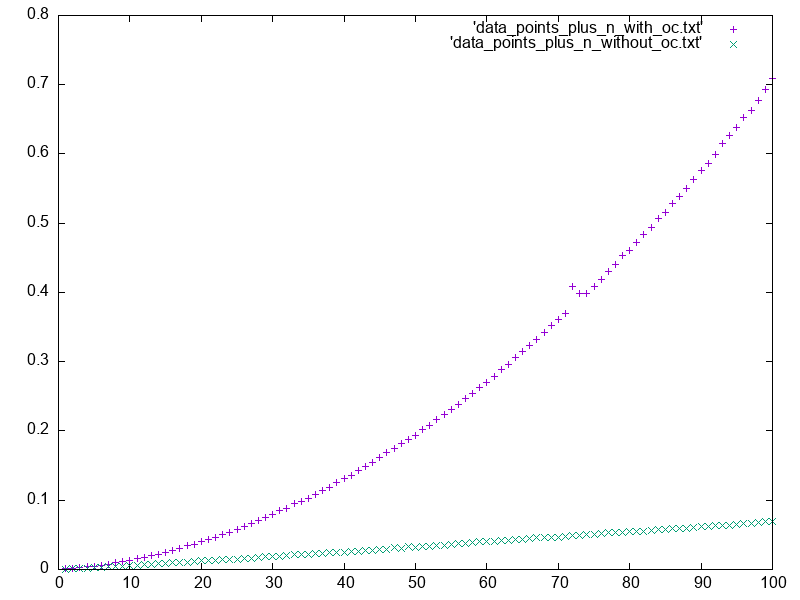
\includegraphics[width=10cm,height=8cm]{plot_example}
  \caption{The graph for the addition query showing the dependency of total time (in seconds) of the search for the query \lstinline|plus$^o$ $\,$ $\overline{n}$ $\,$ $\overline{m}$ $\,$ $r^?$| on the value of $n$ with a fixed $m$. Purple dots show the time for the case when occurs checks are performed, green dots~--- for the case when they are not performed. }
  \label{fig:plot_example}
\end{figure}

To check how well our estimates correspond to the reality we implemented a simple embedding of \mK into \textsc{OCaml} and measured the time of the search for the example queries,
building graphs for the time vs. parameters in the estimated complexity (distinct plot for each parameter).~\footnote{The implementation and the results of the measuring can be found at \url{https://www.dropbox.com/sh/ciceovnogkeeibz/AAAoclpTSDeY3OMagOBJHNiSa}} The referenced embedding follows the standard \textsc{microKanren} implementation but with standard library maps for substitutions and with possibility to switch occurs check on and off.
For time measuring we used standard \textsc{OCaml} library \textsc{benchmark}. The precision we were able to achieve is rather limited, so the plots are not always smooth and can have
deviations (especially for small sizes of the input), but the overall trend is usually clear. Because of the problems with precision, for now we are able to adequately measure only the total
time of the search, with or without occurs check, so we are basically verifying only the \figureword~\ref{fig:examples_total_times}. 
The example of the resulting graph is shown in \figureword~\ref{fig:plot_example} (the time of addition of two numbers depending on the first argument). The character of a time dependency function
is not always visible from the graph (when the degree of the polynomial is greater than one), but after studying each graph individually (for example, by placing the plot between two polynomials of the same degree) we are reasonably convinced that all the complexity estimates from the \figureword~\ref{fig:examples_total_times} are confirmed.

\input{conclusion}

%\section{Appendix}
%\input{lst}

\begin{comment}
%% Acknowledgments
\begin{acks}                            %% acks environment is optional
                                        %% contents suppressed with 'anonymous'
  %% Commands \grantsponsor{<sponsorID>}{<name>}{<url>} and
  %% \grantnum[<url>]{<sponsorID>}{<number>} should be used to
  %% acknowledge financial support and will be used by metadata
  %% extraction tools.
  This material is based upon work supported by the
  \grantsponsor{GS100000001}{Russian Foundation for Basic Research}{https://www.rfbr.ru/rffi/eng} under Grant
  No.~\grantnum{GS100000001}{18-01-00380} and by the grant from JetBrains Research.
  %Any opinions, findings, and
  %conclusions or recommendations expressed in this material are those
  %of the author and do not necessarily reflect the views of the
  %National Science Foundation.
\end{acks}
\end{comment}

\bibliography{references}

\end{document}
